\documentclass[UTF8, xcolor=table]{beamer}
%\usepackage{fontspec}
%\setsansfont{宋体}
\usepackage[BoldFont,SlantFont]{xeCJK}
\setCJKmainfont[BoldFont={SimHei},ItalicFont={KaiTi}]{SimSun}

\usepackage{latexsym,amssymb,amsmath,amsbsy,amsopn,amstext,xcolor,multicol}
\usepackage{graphicx,wrapfig,fancybox}
\usepackage{pgf,pgfarrows,pgfnodes,pgfautomata,pgfheaps,pgfshade}
\usepackage{thubeamer}
\usepackage[backend=bibtex,style=IEEE,sorting=none]{biblatex} % [参考文献格式](https://www.sharelatex.com/blog/2013/07/31/getting-started-with-biblatex.html)
\usepackage{array}
\usepackage{bm}
\usepackage{caption}
\usepackage[caption=false]{subfig}
\usepackage{multirow}
\usepackage{booktabs}

\defbibheading{bibliography}[\bibname]{} %avoid printbibliography 自动生成目录
\addbibresource{ref/papers-bib-in-google.bib}
\addbibresource{ref/chinese-ref.bib}
%\setbeamertemplate{bibliography item}{\insertbiblabel} %将列表中默认的丑陋的icon 改成数字,或者下面这个也行
\setbeamertemplate{bibliography item}[text] % [ref](http://tex.stackexchange.com/questions/68080/beamer-bibliography-icon)
%\setbeamertemplate{footline}[frame number]{}

%\setframeofframes{of}

\usepackage{boxedminipage} %for: bvh border
\def\fourgraphicswidth{0.45} %0.3\textwidth

\usepackage{algorithm} %%format of the algorithm
\usepackage{algpseudocode}
\floatname{algorithm}{算法}
\renewcommand{\algorithmicrequire}{\textbf{输入:}} %%Use Input in the format of Algorithm
\renewcommand{\algorithmicensure}{\textbf{输出:}} %%UseOutput in the format of Algorithm
%\algrenewcommand{\algorithmiccomment}[1]{\hskip3em $\rightarrow$ #1}
\algrenewcommand{\algorithmiccomment}[1]{ $//$ #1}

\usepackage{listings}
\renewcommand\lstlistingname{代码}
\renewcommand\lstlistlistingname{代码}

\lstset{framexleftmargin=1.4em,
        xleftmargin=1.8em,
        basicstyle=\ttfamily\small,
        %frame=shadowbox, numberstyle=\tiny, breaklines=true,
        frame=single,
        numberstyle=\tiny, breaklines=true,
        keywordstyle=\color{blue!70}\bfseries,
        %commentstyle=\color{red!50!green!50!blue!50},
        rulesepcolor=\color{red!20!green!20!blue!20},
        numbers=none,fontadjust=true}
\lstdefinelanguage{shader}{morekeywords={uniform, layout, uniform, vec2, vec3, vec4, in, out, gl_Position, dot, flat, int ,float, gl_VertexID, xyz, w, x, y, z, location, version, sampler2DRect, bgr, gl_FragData, texture2DRect, gl_TexCoord,for,xy},morecomment=[l]{//}}

\begin{document}

\setbeamerfont{footnote}{size=\tiny}
\setbeamerfont{caption}{size=\scriptsize}
\setbeamertemplate{caption}[numbered]

\graphicspath{{figures/}}

\title{凸包围多面体生成算法及应用}
%\author{唐磊}
\author[唐磊]{(申请清华大学工学硕士学位论文答辩报告)\vskip 20pt研~究~生:唐~~~~~磊~~~~~\vskip 5pt 指导教师:雍~俊~海~教授}
\institute[清华大学~软件学院~CG~\&~CAD~研究所]{\small \vskip 38pt计算机辅助设计图形学与可视化研究所}
%\date{2015-06-07}
\date{\small \vskip -17pt二〇一五年六月}
%\date{\today}



\frame{
\vspace{-15mm}
\titlepage
\vspace{-43mm}
\begin{figure}[htbp]
  \begin{center}
	
\includegraphics[width=0.16\linewidth]{Tsinghua_University_Logo.eps}
  \end{center}
\end{figure}
%\beign{picture}(1,1)
%\put(6,8){
\includegraphics[width=0.15\linewidth]{Tsinghua_University_Logo.eps}}
%\end{picture}
}

  \section*{目录}
  \frame {
    \frametitle{\secname}
    \tableofcontents
  }

  \AtBeginSubsection[] {
  \frame<handout:0> {
  \frametitle{目录}
  \tableofcontents[current,currentsubsection]
    }
  }

  \section{引言}
  \frame
  {
    \frametitle{\secname~ }
    \begin{block}{凸包围体技术}
      在计算机图形学领域里的各种算法中发挥着重要作用,
      如优化渲染和建模过程,加速求交、碰撞检测等算法。
    \end{block}

    \begin{block}{碰撞检测问题}
   计算机图形学、虚拟现实等领域中的研究热点,
   是计算机模拟真实环境中不可或缺的技术,
   在物理仿真及游戏领域里应用十分广泛。
    \end{block}
  }

  \subsection{凸包围体}
  \frame{
  \frametitle{凸包围体的种类}
  \begin{figure}
  \hspace{-2.0em}
    \begin{minipage}{1.06\textwidth}
    \subfloat[\scriptsize AABB]
        {
           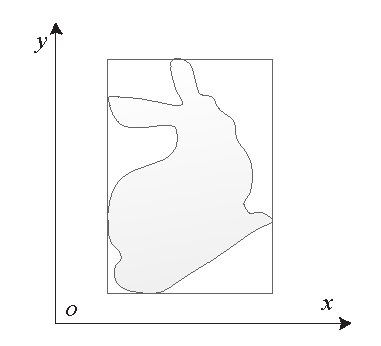
\includegraphics[width=0.2\textwidth]{figures/bunny-2d-AABB.eps}
        }
        \subfloat[\scriptsize OBB]
        {
            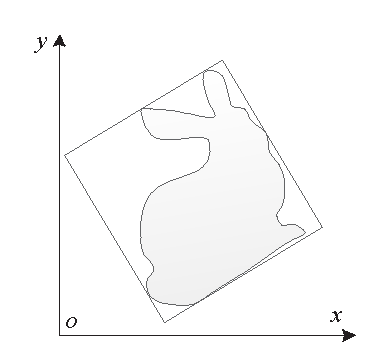
\includegraphics[width=0.2\textwidth]{figures/bunny-2d-OBB.eps}
        }
       \subfloat[\scriptsize Sphere]
        {
           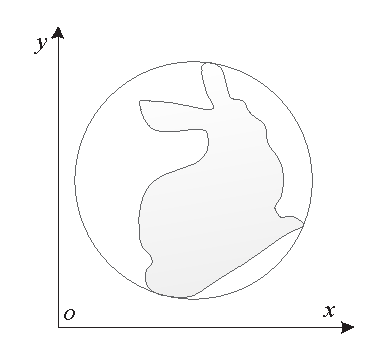
\includegraphics[width=0.2\textwidth]{figures/bunny-2d-Sphere.eps}
        }%\linebreak
        \subfloat[\scriptsize $k$-DOP]
        {
           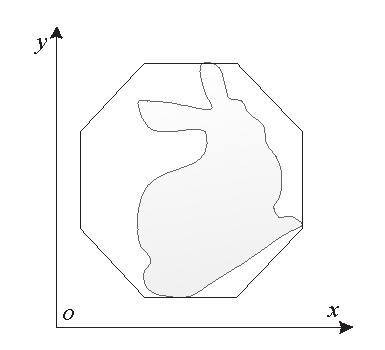
\includegraphics[width=0.2\textwidth]{figures/bunny-2d-8DOP.eps}
        }
        \subfloat[\scriptsize 凸包]
        {
           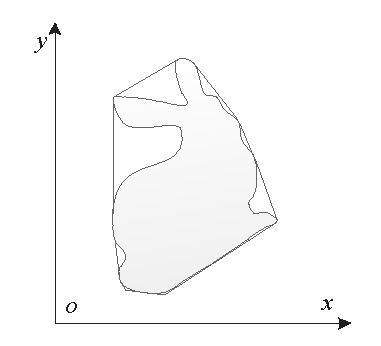
\includegraphics[width=0.2\textwidth]{figures/bunny-2d-Convexhull.eps}
        }
        \end{minipage}
        \caption{不同种类的包围体}
        \label{chart:exps:tightness}
        \end{figure}
        \vspace{-1em}
      其他:Tribox、Swept-sphere、 Sphere-shell、Zonotopes、圆柱形、圆锥、椭球形等等。
  }

      \frame{
   \frametitle{本文目标}
   \begin{block}{综合比较}
   \begin{description}
     \item[$k$-DOP\cite{klosowski1998efficient}:]方向固定且有限,不同模型其截面方向一致, 不够紧致。
     \item[凸包:]很(最)紧致, 但面片数量太多, 复杂度$O(n\log n)$。
    \end{description}
  \end{block}
  \begin{block}{本文凸包围体的目标}
     \begin{description}
     \item[紧致:] 能够自适应模型
     \item[快速:] 利用~GPU~加速
     \item[灵活:] 通过参数~$k$~调节简单性和紧致性
     \end{description}
   \end{block}
  }

  \subsection{碰撞检测算法}
   \frame{
   \frametitle{\subsecname~ }
    
   \begin{block}{碰撞检测算法}
    许多应用的基础,例如在~3D~游戏,物理仿真,机器人,虚拟现实等领域中。
   \end{block}

   \begin{block}{分类}
     \begin{description}
       \item[加速结构:] SPT(如四叉树、KD~树等)~v.s~BVH(OBB树、$k$-DOP树等)
       \item[表现形式:] 刚体~v.s~可变形,凸体~v.s~凹体,CSG~v.s~参数曲面~v.s~多边形网格
       \item[碰撞环境:] 成对~v.s~多体,静止~v.s~运动,离散~v.s~连续
     \end{description}
   \end{block}
  }

  \frame{
    \frametitle{基于~BVH~的碰撞检测算法}
    \begin{columns}[onlytextwidth]
      \begin{column}{0.35\textwidth}
        \vspace{-1.5em}
        \begin{figure}[htbp]
            \begin{center}
            \begin{boxedminipage}{1\textwidth}
            \subfloat{\label{lbl:bvh-bunny-center-0.png}}
              {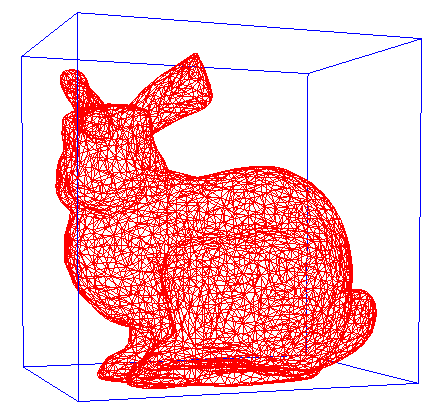
\includegraphics[height=1.4cm]{bvh-bunny-center-0.png}}
            \subfloat{\label{lbl:bvh-bunny-center-1.png}}
              {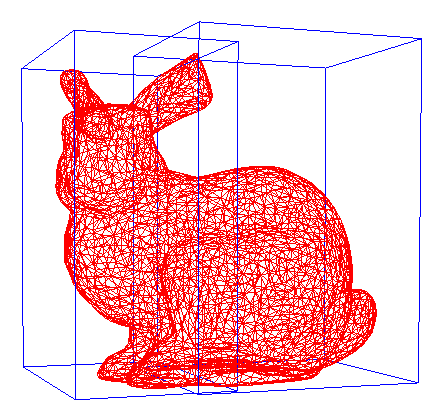
\includegraphics[height=1.4cm]{bvh-bunny-center-1.png}}
            \\
            \subfloat{\label{lbl:bvh-bunny-center-2.png}}
              {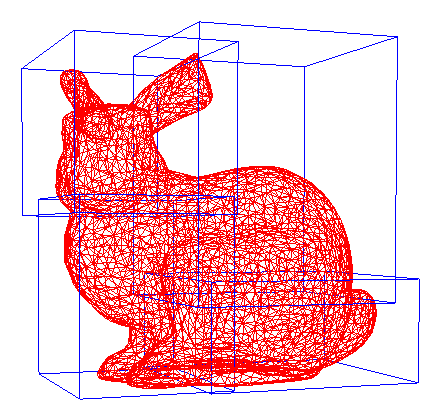
\includegraphics[height=1.4cm]{bvh-bunny-center-2.png}}
            \subfloat{\label{lbl:bvh-bunny-center-3.png}}
              {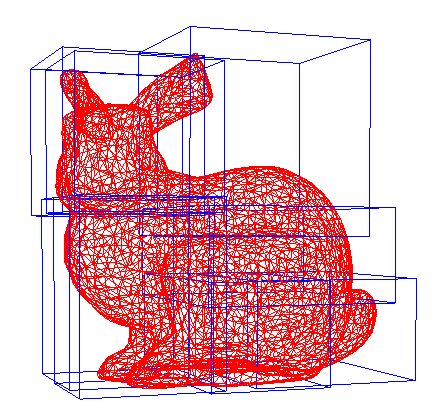
\includegraphics[height=1.4cm]{bvh-bunny-center-3.png}}
            \\\hspace{0.5cm}
            \subfloat{\label{lbl:bvh-bunny-center-4.png}}
              {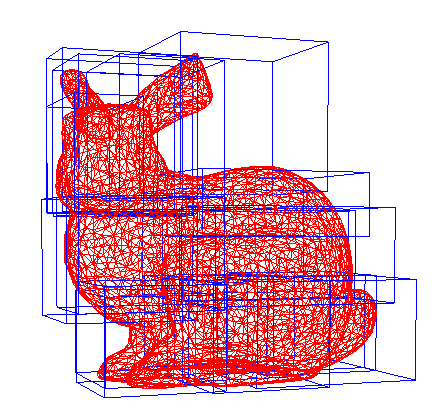
\includegraphics[height=1.5cm]{bvh-bunny-center-4.png}}
            \subfloat{\label{lbl:bvh-bunny-center-5.png}}
              {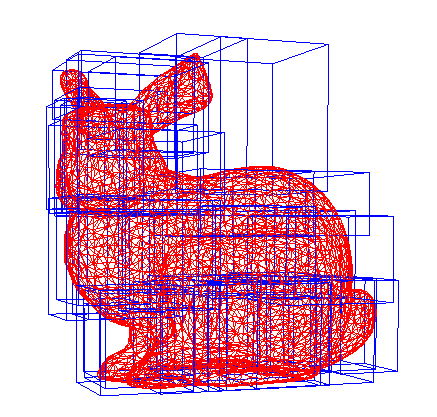
\includegraphics[height=1.5cm]{bvh-bunny-center-5.png}}
            \\
            \subfloat{\label{lbl:bvh-bunny-center-6.png}}
              {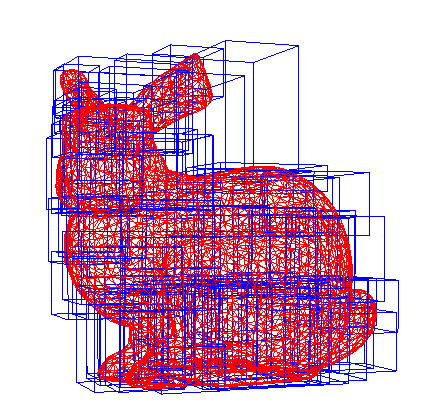
\includegraphics[height=1.5cm]{bvh-bunny-center-6.png}}
            \subfloat{\label{lbl:bvh-bunny-center-7.png}}
              {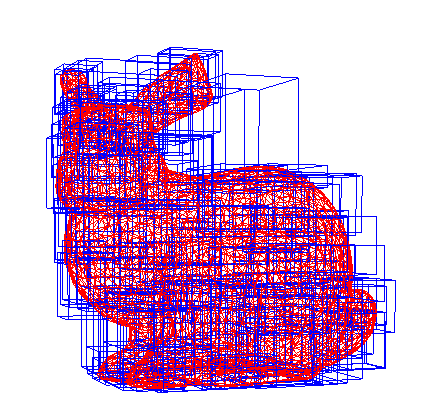
\includegraphics[height=1.5cm]{bvh-bunny-center-7.png}}
            \end{boxedminipage}
            \vspace{-0.5em}
          \caption{八层~BVH~示例}
          \label{lbl:bvh-example}
          \end{center}
          \end{figure}
      \end{column}
      \hspace{0.5em}
      \begin{column}{1.2\textwidth}
      \vspace{0.2em}
         \scalebox{0.5}{
              \begin{minipage}{1.0\textwidth}
      \vspace{-2em}
           \begin{algorithm}[H]
              \caption{自顶向下层次遍历~BVH~}
              \label{alg:traverse-bvh-tree}
              \begin{algorithmic}[1]
              \Require
              两个~BVH~树的根节点~$node_1$,$node_2$
              \Ensure
              模型是否相交
              \Function {TraverseBVHTree}{$node_1, node_2$}
                \If{$node_1.bv \cap node_2.bv = \emptyset$}
                  \State \Return{\textbf{False}}
                  \Comment{包围体重合测试, 包围体不相交直接返回}
                \Else
                    \If {$node_1.children = \emptyset$}
                         \If {$node_2.children = \emptyset$}
                         \State \Comment{最底层叶子节点原生几何相交测试}
                         \State \Return {\Call{CheckIntersection}{$node_1.primitives, node_2.primitives$}}
                         \Else
                            \ForAll {$child \in node_2.children$}
                            \State \Call{TraverseBVHTree}{$node_1, child$} \Comment{递归调用}
                            \EndFor
                         \EndIf
                    \Else
                         \ForAll {$child \in node_1.children$}
                         \State \Call{TraverseBVHTree}{$child, node_2$}  \Comment{递归调用}
                         \EndFor
                    \EndIf
                \EndIf
              \EndFunction
              \end{algorithmic}
              \end{algorithm}
              \end{minipage}
            }
      \\
      %\begin{block}{代价函数}
      \scriptsize \hspace{1em}代价函数: $T_{cost} = n_v * C_v + n_p * C_p + (n_u * C_u)$(运动)
      %\end{block}
      \end{column}
    \end{columns}
}


  \section{模型适应的凸包围多面体构造算法}

    \subsection{问题定义及算法流程}

     \frame{
       \frametitle{问题的定义}
      \begin{columns}[onlytextwidth]
          \begin{column}{0.7\textwidth}
           \begin{block}{凸包围~$k$~面体}%
            $k$-Convex Bounding Polyhedron,简称~$k$-CBP,可通过~$k$~个半空间定义:
              \begin{equation}
              \label{equ:kcbp_definition}
              \left\{
                \begin{array}{l}
                    k\mbox{-CBP} = \mathop  \bigcap \limits_{i = 1}^k \bm{H_i} \\
                    \bm{H_i} = \left\{ {\left. {\bm{p} \in {\mathbb{R}^3}} \right| \bm{n_i} \cdot \bm{p} \le {w_i}} , w_i \in \mathbb{R} \right\},
                \end{array}
              \right.
              \end{equation}
              其中,$\bm{n_i}$~是半空间~$\bm{H_i}$~的法向,方向指向包围体外部,
              $w_i$~是输入点集中沿~$\bm{n_i}$~方向投影的最大值。
           \end{block}
    %        \pgfputat{\pgfxy(5,0)}{\pgfbox[left,top]{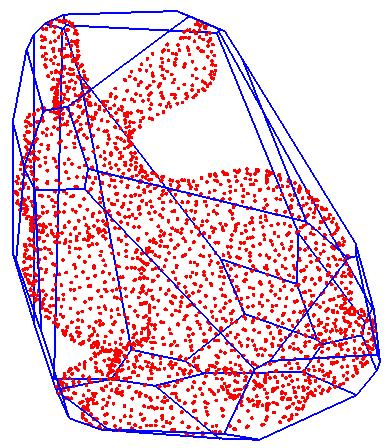
\includegraphics[width=0.25\textwidth]{bunny-34.png}}}
        \end{column}

       %\pgfputat{\pgfxy(7,-1.5)}{\pgfbox[left,top]{
       %  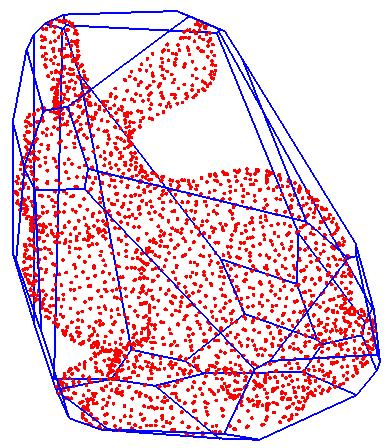
\includegraphics[width=0.25\textwidth]{bunny-34.png}
       %}}
        \begin{column}{0.4\textwidth}
        \begin{figure}
            %\pgfputat{\pgfxy(7,-1.5)}{\pgfbox[left,top]{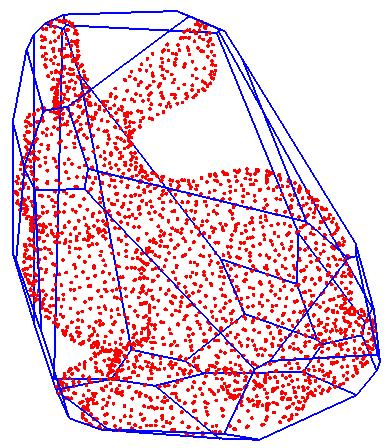
\includegraphics[width=0.8\textwidth]{bunny-34.png}}} %%cannot use caption for pgfputat
            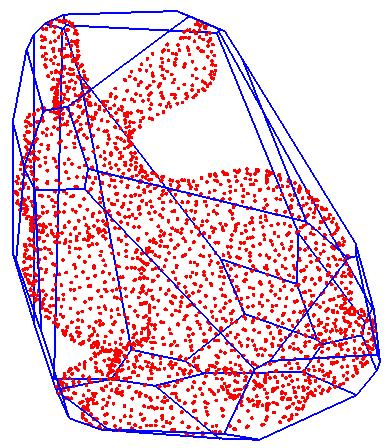
\includegraphics[width=0.8\textwidth]{bunny-34.png}
            \caption{34-CBP}
        \end{figure}
        \end{column}
      \end{columns}
    }

       \frame{
       \frametitle{算法流程}
       \begin{block}{构造$k$-CBP~算法流程图}
        \begin{figure}
        \centering
        %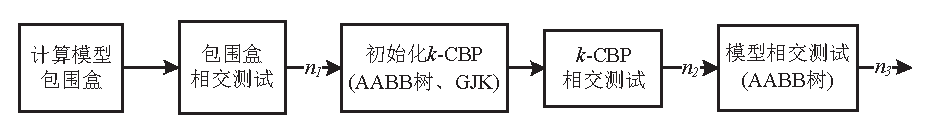
\includegraphics[width=4.0in]{figures/collision-detection-flowchart.eps}
        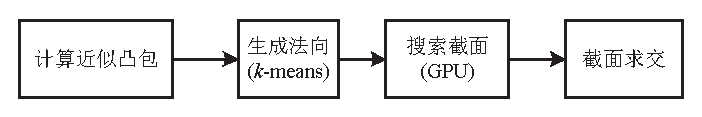
\includegraphics[width=4.0in]{kcbp-flowchart-x-aix.eps}
        %\caption{构造$k$-CBP~算法流程图}
        \label{lbl:kcbp-algorithm-flowchart}
        \end{figure}
     %   \hspace*{.1\linewidth}
     %   \begin{minipage}{\textwidth}
     %     \begin{exampleblock}{关键步骤}
     %     \begin{description}
     %        \item[定法向:]结合近似内凸包和~$k$-means~
     %        \item[搜截面:]GPU~中沿各法向搜索切点构造截面
     %        \item[求交点:]截面对偶映射求得交点
     %     \end{description}
     %   \end{exampleblock}
     % \end{minipage}
    \end{block}
    \begin{block}{关键步骤}
          \begin{description}
             \item[定法向:]结合近似内凸包和~$k$-means~
             \item[搜截面:]GPU~中沿各法向搜索切点构造截面
             \item[求交点:]截面对偶映射求得交点
          \end{description}
    \end{block}
    }

  \subsection{截面法向的生成}

    \frame{
        \frametitle{近似凸包的构造}
        \begin{figure}
        \vspace{-3mm}
        \subfloat[]
        {
           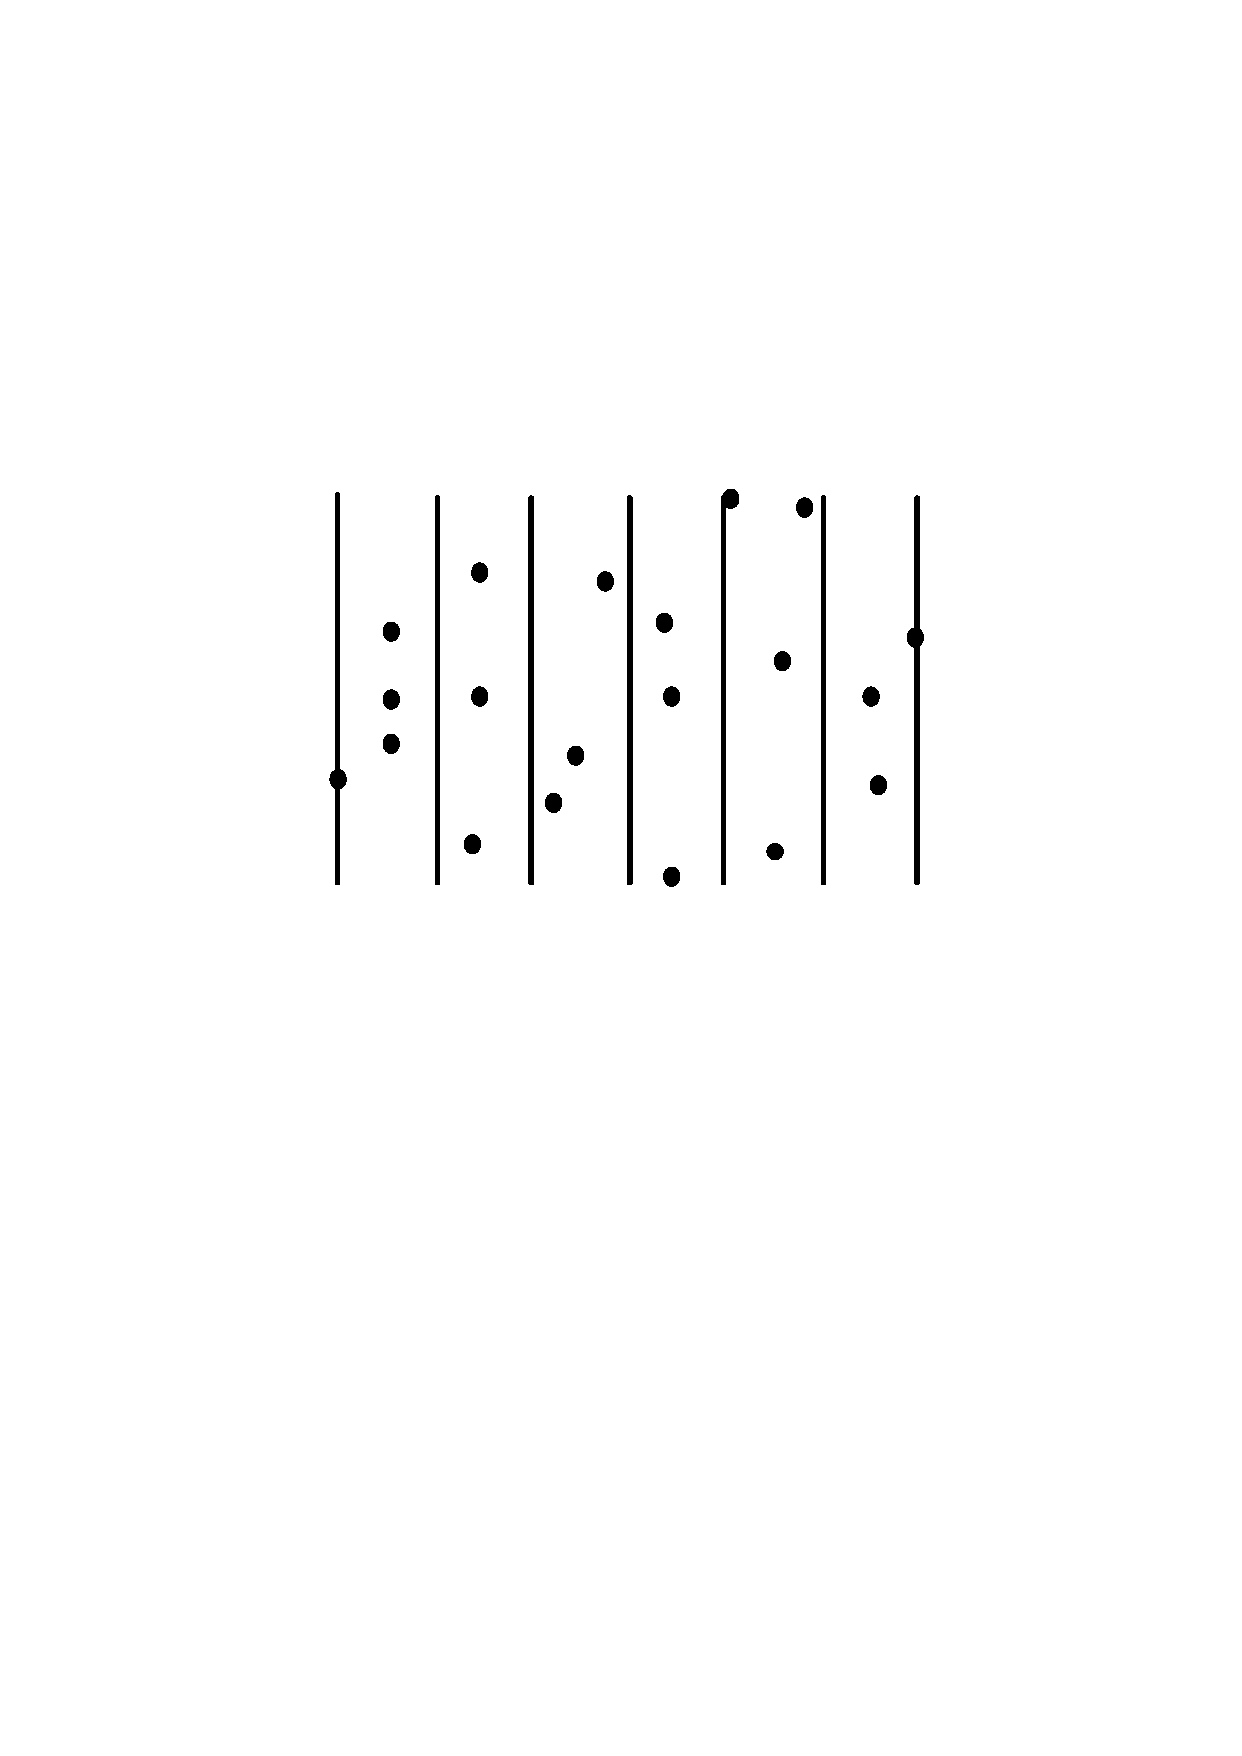
\includegraphics[width=0.28\textwidth]{figures/approximate-convexhull-step1.pdf}
        }\hspace{2mm}
        \subfloat[]
        {
            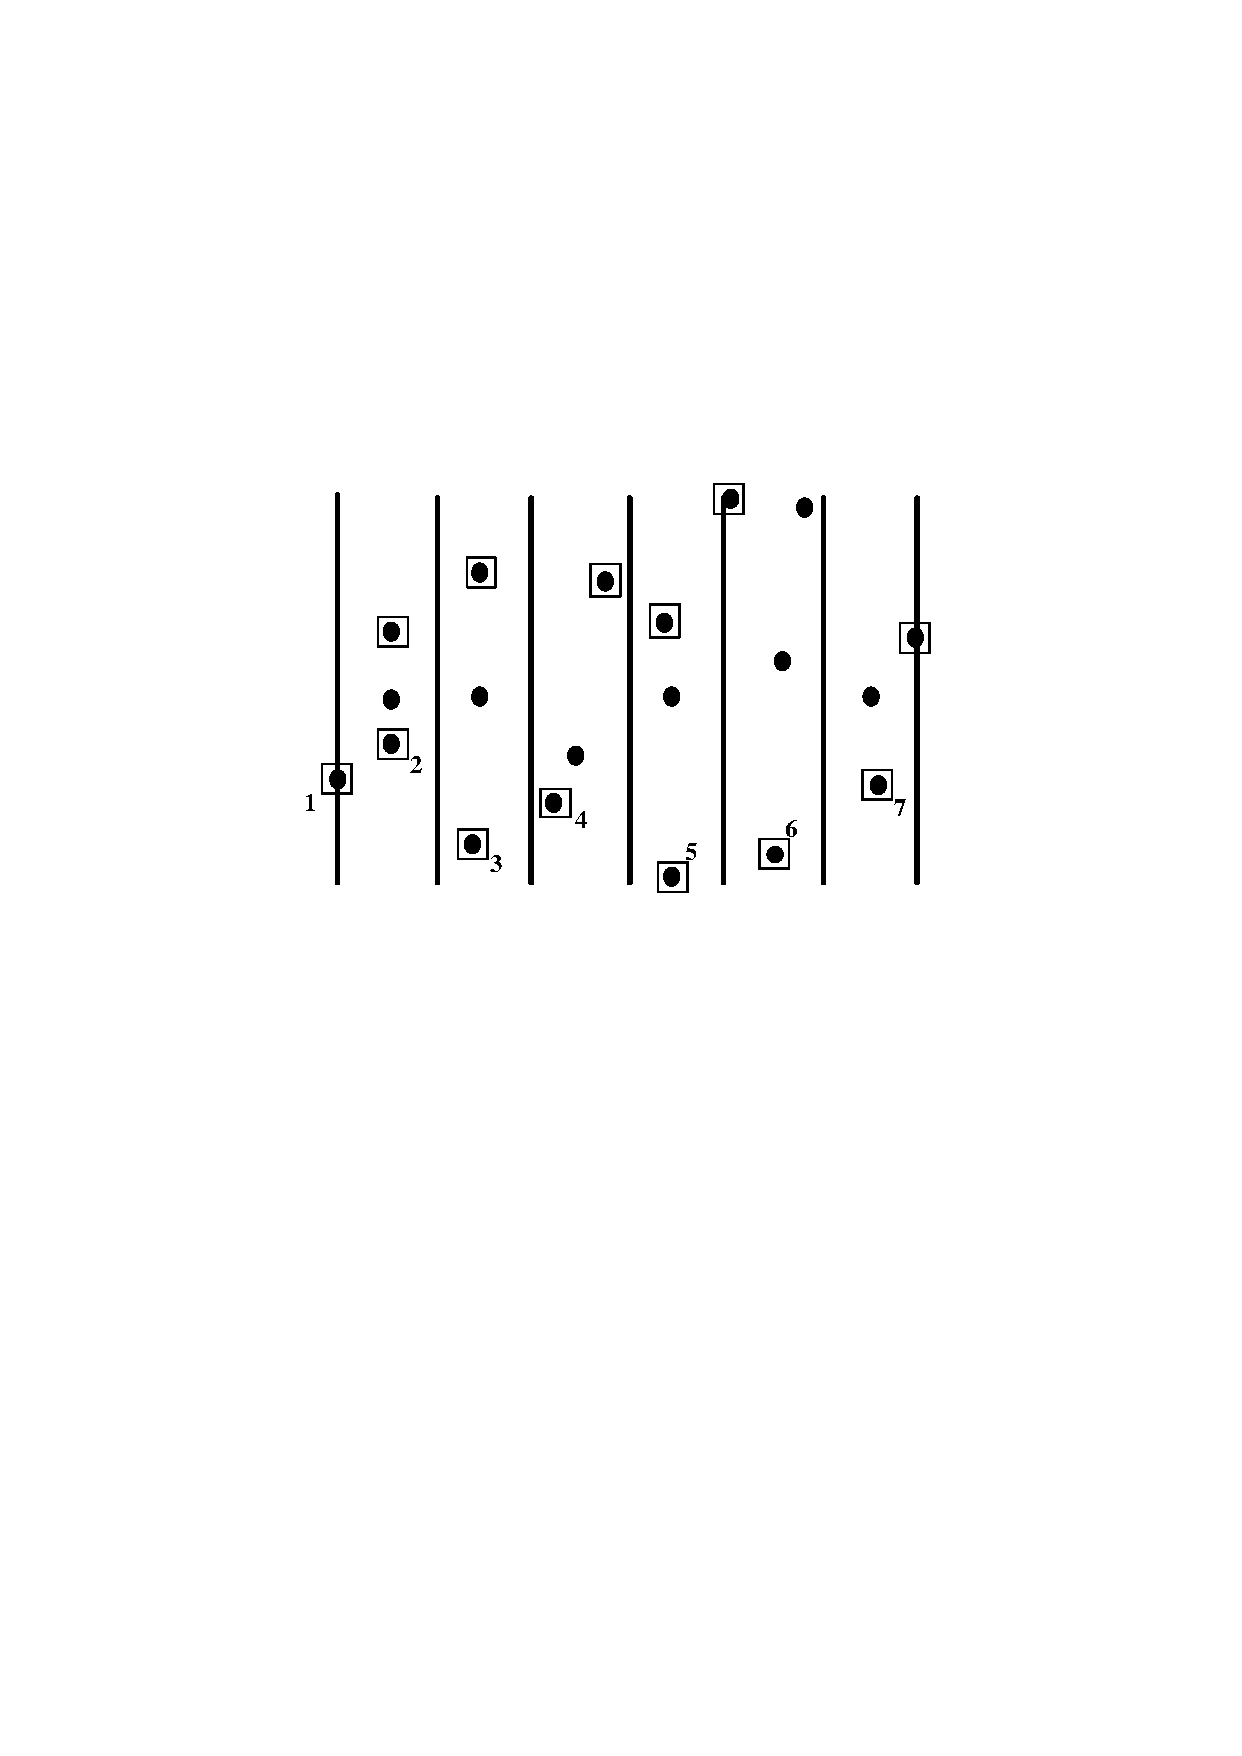
\includegraphics[width=0.28\textwidth]{figures/approximate-convexhull-step2.pdf}
        }\hspace{2mm}
        \subfloat[]
        {
           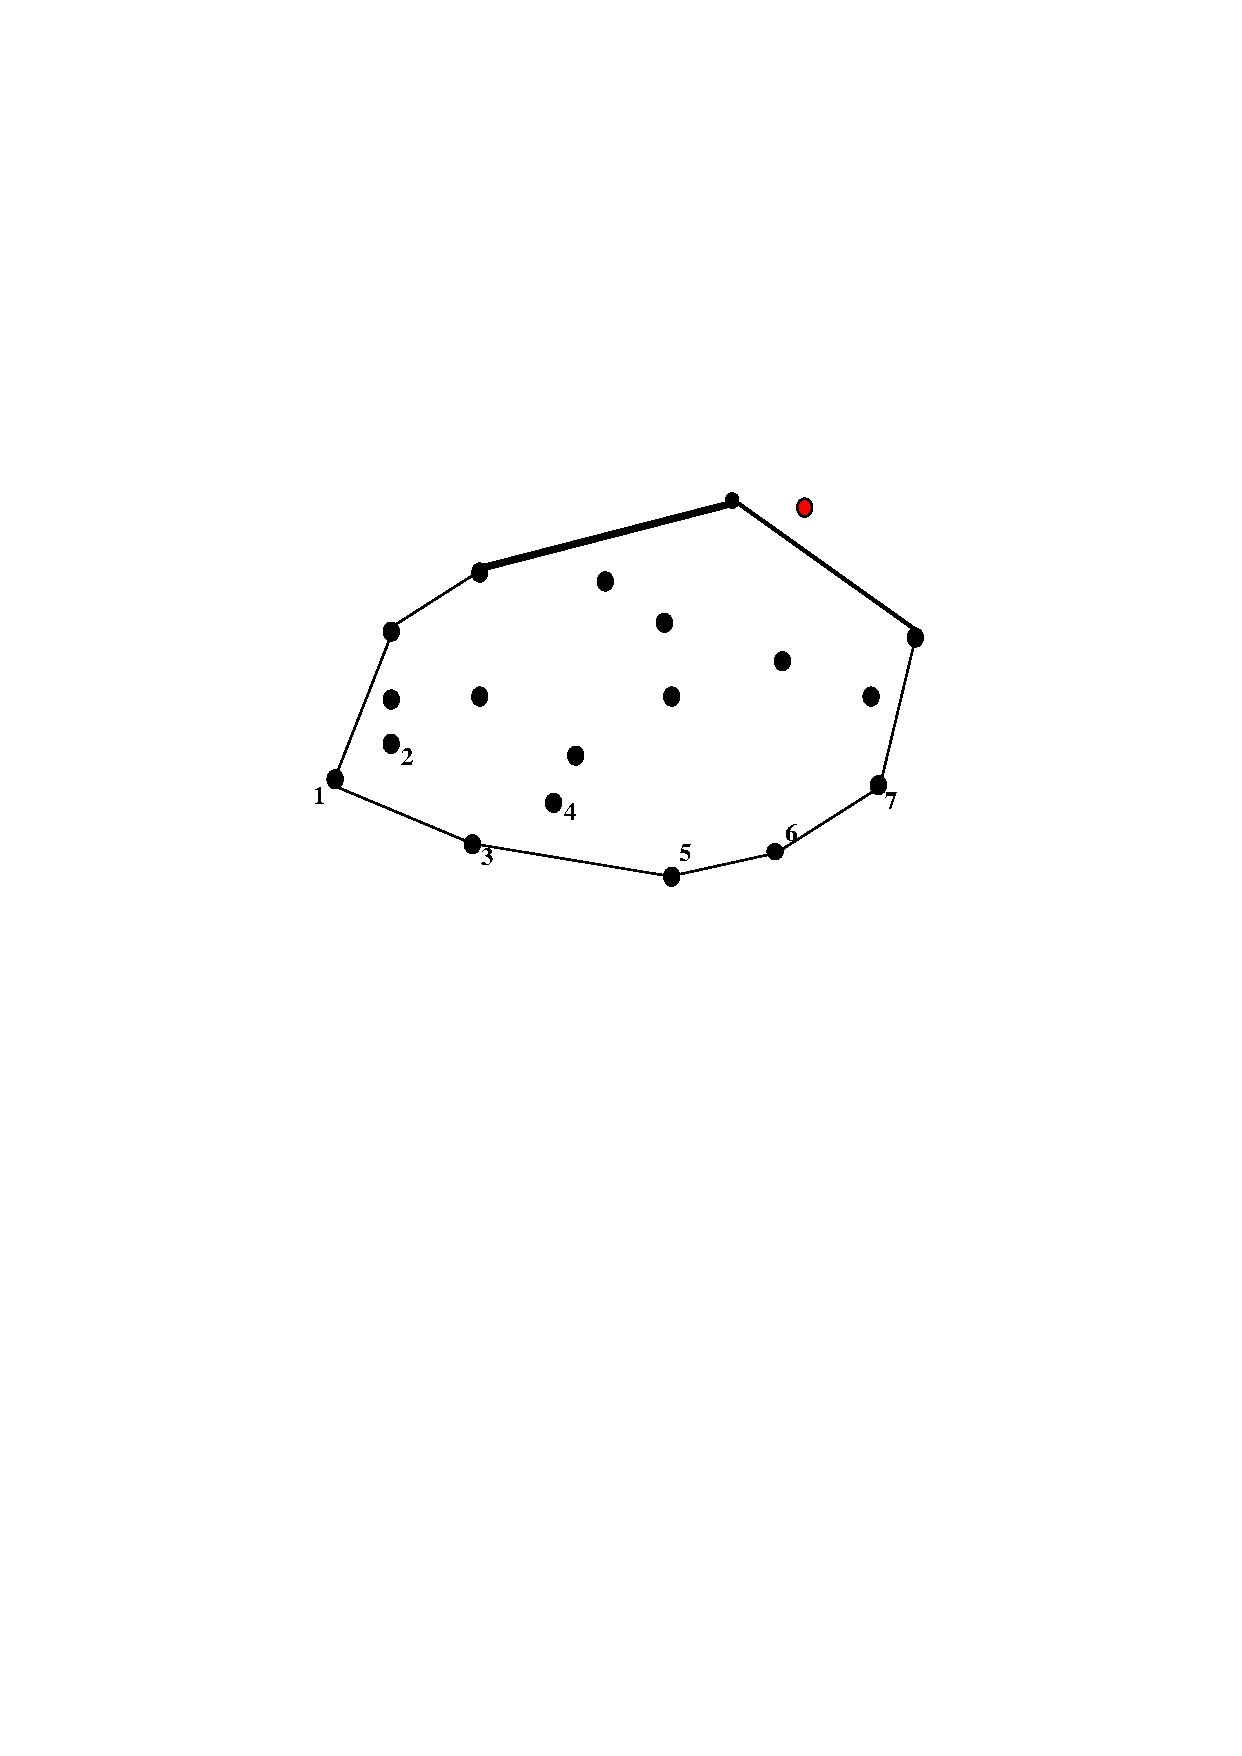
\includegraphics[width=0.28\textwidth]{figures/approximate-convexhull-step3.pdf}
        }
        \caption{二维近似内凸包的构造}
        \label{lbl:ach-2d}
        \end{figure}
        \vspace{-4mm}
        构造近似内凸包\cite{bentley1982approximation}, 算法复杂度为~$O(n+\xi)$, 扩展到三维为~$O(n+\xi^2\log\xi)$, 然后利用 $k$-means 聚类.
    }
    \frame{
        \frametitle{$k$-means 聚类}

        \begin{figure}
        \vspace{-5mm}
        \subfloat[]
        {
           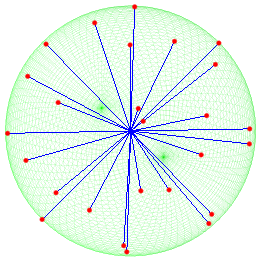
\includegraphics[width=0.28\textwidth]{figures/kmeans-init-normals-26.png}
        }
        \subfloat[]
        {
            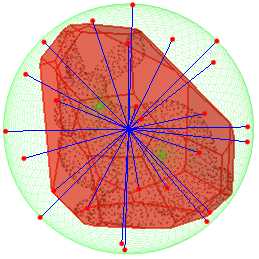
\includegraphics[width=0.28\textwidth]{figures/kmeans-init-normals-26-for-bunny.png}
        }
        \subfloat[]
        {
           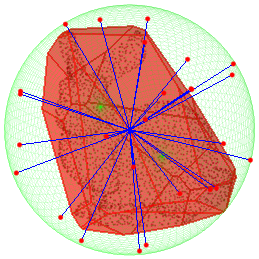
\includegraphics[width=0.28\textwidth]{figures/kmeans-cluster-normals-26-for-bunny.png}
        }
        \vspace{-2mm}
        \caption{通过聚类确定法向}
        \label{lbl:gen-fixed-normals}
        \end{figure}

        \vspace{-6mm}
        \small
        聚类初始方向(均匀分布). 距离度量(余弦), 聚类更新中心点时将面片的面积作为权重即$\bm{c_i}=\frac{\sum_{i=1}^{i=n} \omega_i \cdot \bm{n_i} } {\sum_{i=1}^{i=n} \omega_i}$, 其中$\bm{c_i}$ 为第~$i$~类的中心点, $\omega_i$~ 为法向~$\bm{n_i}$~所在面片对应的面积.
    }

  \subsection{搜索截面及求交}

    \frame{
    \frametitle{搜索截面}
     \footnotesize 等效于寻找最大投影值, 即对每个法向~$\bm{n_i}$, 从输入模型的所有点中寻找最大投影值的点作为切点进而确定~$\bm{n_i}$~对应的截面.
时间复杂度为~$O(k\cdot n)$, 其中~$k$~为法向数量, $n$~为模型所含点数. 各法向的计算相互独立, 借助~GPU~并行加速.

    \begin{figure}
    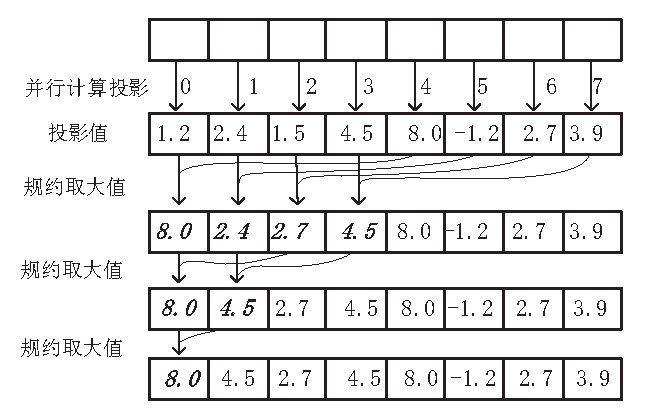
\includegraphics[width=2.5in]{figures/gpureduction.eps}
    \caption{并行规约求最大投影值}
    \label{lbl:reduction-getmax}
    \end{figure}
    }

        \frame{
    \frametitle{求交算法}
      \small 法向~$\bm{n}(a,b,c)$~及平面上一点~$\bm{p}(x_0,y_0,z_0)$~确定, 转化为平面方程~$ax + by + cz = ax_0 + by_0 + cz_0=d$, $d \neq 0$. 对偶映射后的点为~$\bm{p'}(a/d, b/d, c/d)$, 对这~$k$~个映射点求凸包, 凸包平面映射回原来的交点, 时间复杂度为$O(k\log k$).

      亦可直接通过枚举所有每~3~个平面交于~1~点的情况, 然后排除在平面外部的交点, 剩下的构成~$k$-CBP~的顶点, 时间复杂度为$O(k^3$)\cite{ericson2005real}.
    }


  \section{实验与分析}

  \subsection{凸包围多面体的生成速度}

    \frame{
        \begin{figure}
         \vspace{-5mm}
        \subfloat%[Budda(31232 points)]
        {  \label{fig:exp:cpu:budda}
           \includegraphics[width=0.38\textwidth,page=2]{figures/cudatime.pdf}
        }
        \subfloat%[Dinosaur(40277 points)]
        {  \label{fig:exp:cpu:Dinasour}
            \includegraphics[width=0.38\textwidth, page=3]{figures/cudatime.pdf}
        }\linebreak %强制换行
        \vspace{-5mm}%
       \subfloat%[Alice(224291 points)]
        {  \label{fig:exp:cpu:alice}
           \includegraphics[width=0.38\textwidth, page=4]{figures/cudatime.pdf}
        }
        \subfloat%[Bugatti(1010815 points)]
        {  \label{fig:exp:cpu:buggatti}
           \includegraphics[width=0.38\textwidth, page=5]{figures/cudatime.pdf}
        }
        \caption{本文算法与~CPU~算法对比\tiny Budda(31k),Dinosaur(40k),Alice(224k), Bugatti(1011k)}
        \label{chart:exps:cputime}
        \end{figure}
    }

    \frame{
        图~\ref{chart:exps:cputime} 中横纵坐标分别代表多面体面数和运行时间, 其中虚线代表搜索截面的过程, 实线为构造凸包围多面体总体耗时. 当模型点数量较大时, 搜索截面的过程占据了算法绝大多数时间, 且随着凸包围多面体的面数~$k$~ 值增加而线性增长, 这与搜索截面时间复杂度($O(k\cdot n)$)一致, 截面求交过程的时间复杂度为$O(k\log k)$,
当点数量极大时, 实线虚线几乎重合即求交等步骤耗时相比整体算法而言几乎可忽略.
    }

    \frame{
     \vspace{-7mm}
        \begin{table} \tiny
        \caption{本文算法与文献\cite{karlsson2010parallel}算法对比}
        %\centerline{\zihao{-5}\bf \small 表1\quad 本文算法与文献~${[21]}$~算法对比}
        %\centerline{\footnotesize{\bf Table 1}\quad Comparison of result between ${[21]}$ and ours}
        %\begin{center}\belowrulesep=0pt\renewcommand{\arraystretch}{1.3} \doublerulesep 0.4pt \tabcolsep 15pt
        \begin{tabular}{p{1.5cm}<{\centering}ccc ccc} %p本身占一列
        \hline
        \multirow{2}{*}{$k$} & \multicolumn{3}{c}{Apple(8118 points)} & \multicolumn{3}{c}{~~~~~Bugatti(1010815 points)}\\
        %\cmidrule(lr){2-4}\cmidrule(lr){5-7}
        %\hline
        %\rowcolor[gray]{0.9} $k$ &
        ~&SSE$^{5}(ms)$ & $k$-CBP(ms) &  Speedup &SSE(ms) & $k$-CBP(ms) &  Speedup \\
        \hline
        6 & 0.4 & 0.12  & 3.20     & 24.2 & 3.20  & 7.56 \\
        16 & 0.9 & 0.26  & 3.43    & 44.5 & 8.44  & 5.27 \\
        26 & 1.4 & 0.41  & 3.38    & 66.5 & 13.65  & 4.87 \\
        36 & 1.9 & 0.52  & 3.65    & 91.1 & 18.34  & 4.97 \\
        46 & 2.5 & 0.67  & 3.74    & 119.5 & 24.13  & 4.95 \\
        56 & 2.9 & 0.79  & 3.66    & 138.4 & 28.86  & 4.80 \\
        66 & 3.5 & 0.95  & 3.69    & 170.6 & 34.10  & 5.00 \\
        76 & 4.0 & 1.08  & 3.70      & 197.1 & 39.85  & 4.95 \\
        86 & 4.5 & 1.22  & 3.69    & 219.8 & 45.08  & 4.88 \\
        106 & 5.4 & 1.49  & 3.62   & 267.8 & 55.52  & 4.82 \\
        136 &  6.8 & 1.92  & 3.54  & 342.9 & 71.24  & 4.81 \\
        156 &  7.7 & 2.17  & 3.55  & 411.3 & 81.18  & 5.07 \\
        186 &  9.3 & 2.60  & 3.58  & 479.4 & 97.39  & 4.92 \\
        206 &  10.5 & 2.85  & 3.68 & 523.0 & 106.87  & 4.89  \\  \hline
        \end{tabular}
        \label{tab:exp:sse-time}
        \end{table}
        \vspace{-3mm}
    \scriptsize 点数量较小时, 能够提高~3-4~倍速度,模型变大, 加速比更大, ~Bugatti~模型的提速达到~4-8~倍.
    }

  \subsection{凸包围多面体的紧致程度}

   \frame{

        \begin{figure}
         \vspace{-5mm}
        \subfloat
        {  \label{fig:exp:cpu:budda}
           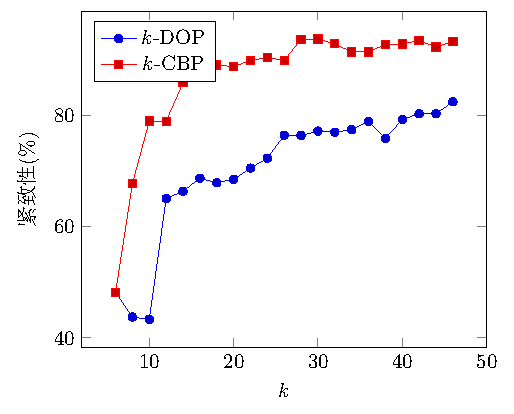
\includegraphics[width=0.35\textwidth,page=1]{figures/tightness.pdf}
        }
        \subfloat
        {  \label{fig:exp:cpu:Dinasour}
            \includegraphics[width=0.35\textwidth, page=2]{figures/tightness.pdf}
        }\linebreak %强制换行
        \vspace{-3mm}%
       \subfloat%[Alice(224291 points)]
        {  \label{fig:exp:cpu:alice}
           \includegraphics[width=0.35\textwidth, page=3]{figures/tightness.pdf}
        }
        \subfloat%[Bugatti(1010815 points)]
        {  \label{fig:exp:cpu:buggatti}
           \includegraphics[width=0.35\textwidth, page=4]{figures/tightness.pdf}
        }
        \caption{紧致程度对比: $k$-DOP v.s $k$-CBP \tiny Apple(8k), Budda(31k), Dinosaur(40k), Alice(224k)}
        \label{chart:exps:tightness}
        \end{figure}
        \vspace{-8mm}
        紧致程度用凸包与凸包围多面体的体积之比来量化.
    }


    \frame{


        \begin{table}
        \scriptsize
        \caption{\label{tab:exp:cgal}$k$-CBP~与~QuickHull~凸包算法比较}
         %\centerline{\zihao{-5}\bf \small 表2\quad $k$-CBP~与~QuickHull~凸包算法比较}
        %\centerline{\footnotesize{\bf Table 2}\quad Comparison of result between QuickHull and $k$-CBP}
        %\vspace{3mm}{\zihao{6}\footnotesize
        %\begin{center}\belowrulesep=0pt\renewcommand{\arraystretch}{1.3} \doublerulesep 0.4pt \tabcolsep 10pt
         \begin{tabular}{lcccccl}
          \toprule
          Model & f(CHull)& f($k$-CBP) & $\tau$ ($k$-CBP) & t(CHull(ms)) & t($k$-CBP(ms))\\ % 后面重新跑的, KCBP加上了近似凸包及求交时间的总和, 和近似凸包的分组时间也加了.
          \midrule
          Apple	& 499 & 30 & 93.67\% & 5.5 & 1.30\\ % apple3  自己电脑跑的数据, 之前是用的chengxianyu的电脑.
          Budda	& 1608 & 46 & 92.39\% & 21.3 & 2.86 \\ %  1.0+0.86+1
          Dinosaur	& 1240 & 44 & 93.34\% & 22.6 & 1.99 \\  % 1.0+0.98+0.1
          Alice	& 1332 & 44 & 93.92\% & 85.8 & 8.47\\ % 2+6.48
          Bugatti & 24654 & 44 & 95.06\% & 688.7 & 25.41\\
          \bottomrule
         \end{tabular}
         \vspace{-2mm}
        \end{table}

        \small  $\tau$($k$-CBP)~为凸包围多面体的紧致程度. 与凸包相比, 本文算法在大大简化包围体平面数量的同时能保持较好的紧致程度, 下图为可视化结果.
    }

    \frame{
%          \begin{figure}
%    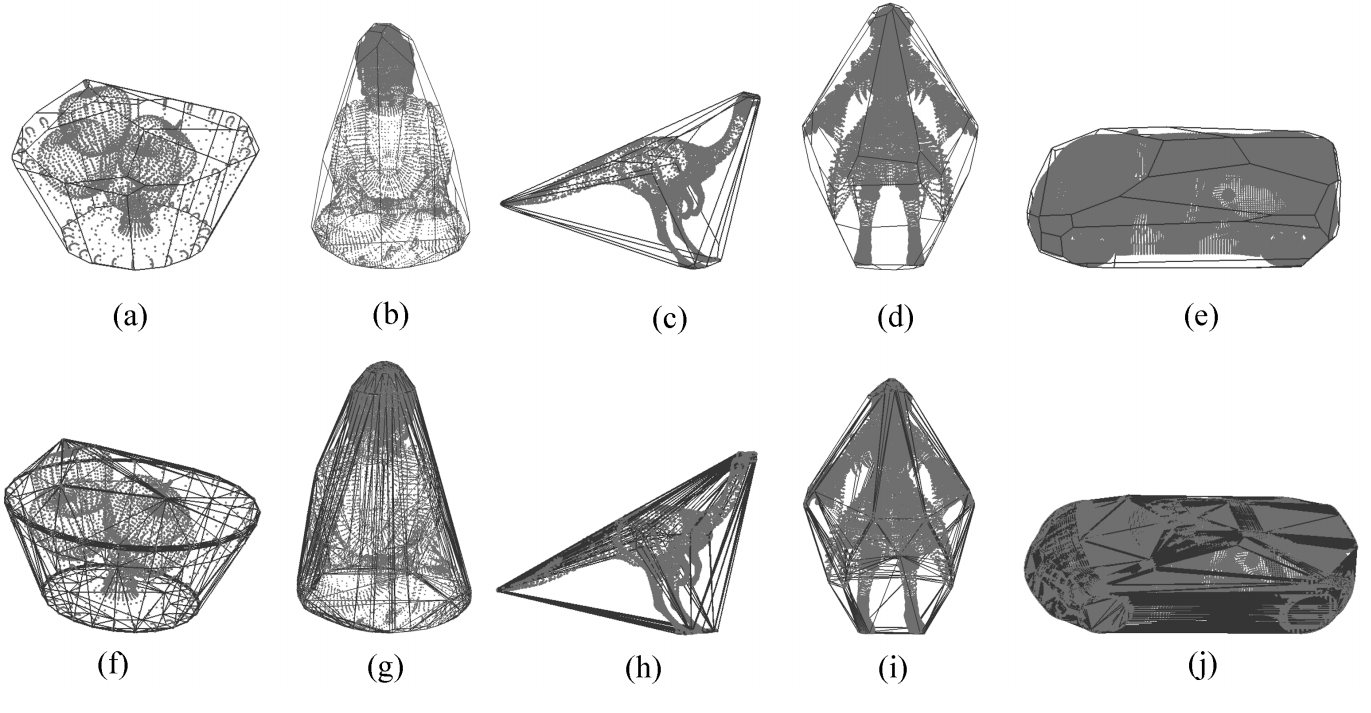
\includegraphics[width=4.0in]{figures/N112014-00019-9}
%    \caption{$k$-CBP~与凸包对比: \tiny (a) Apple (30-CBP); (b) Budda (46-CBP); (c) Dina-
%sour (44-CBP); (d) Alice (44-CBP); (e) Bugatti (44-CBP); (f) Apple (CHull); (g) Budda (CHull); (h) Dinosaur (CHull);
%(i) Alice (CHull); (j) Bugatti (CHull)}
%    \label{pic:exps:ch-kcbp}
%    \end{figure}

    \begin{figure}
    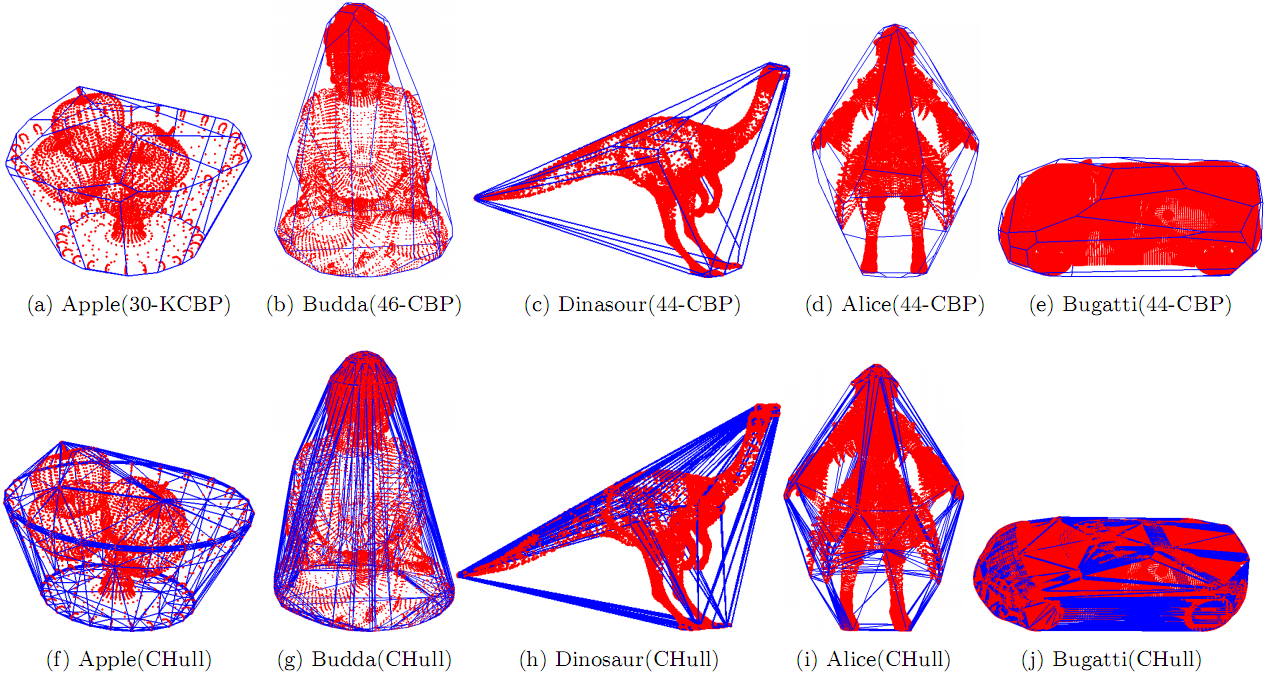
\includegraphics[width=4.0in]{figures/kcbp-convexhull.png}
    \caption{$k$-CBP~与凸包对比}
    \label{pic:exps:ch-kcbp}
    \end{figure}

    }

      \subsection{凸包围多面体的简单应用}

    \frame{
        \begin{figure}
        \centering
        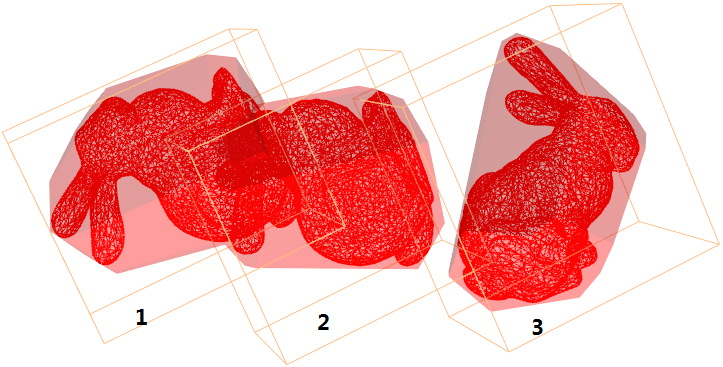
\includegraphics[width=3in]{figures/bunny-box-kcbp-collsion-detection-example.png}
        \caption{~$k-$CBP~应用于碰撞检测示例}
        %\centerline{\bahao\bf 图 10\quad ~$k-$CBP~应用于碰撞检测示例}
        %\centerline{\footnotesize {\bf Figure 10}\quad  Example of collision detection using $k$-CBP}
        \label{lbl:bunny-box-kcbp-collsion-detection-example}
        \end{figure}

        \small 图中模型~1~与~2、2~与~3~的包围盒分别相交, 而其~$16$-CBP~仅~1~与~2~相交, 实际模型仅~1~与~2~相交. 不同数量的模型(模型位置和旋转角度随机生成)测试结果如下表所示.
    }

    \frame{
        \begin{table}
        \tiny
        \centering
         \caption{\label{tab:exp:box:kcbp:collsiondetection}$k$-CBP~和包围盒应用于碰撞检测结果对比}
        % \centerline{\zihao{-5}\bf \small 表4\quad }
        %\centerline{\footnotesize{\bf Table 4}\quad Comparison of result of collision detection between $k$-CBP and bounding box}
        %\vspace{3mm}{\zihao{6}\footnotesize
        %\begin{center}\belowrulesep=0pt\renewcommand{\arraystretch}{1.3} \doublerulesep 0.4pt \tabcolsep 10pt
         \begin{tabular}{lccccccl}
          \toprule
          n& c(Box) & c($16$-CBP) &  t(Box) & t($16$-CBP) & r(Box) & r($k$-CBP) & n(Model) \\
          \midrule
           10 & 0.1 & 1.8 &    26.0  & 0.1    & 0.00 \% &  100.00\% & 0\\
           30 & 0.2 & 2.9 &   134.0  & 70.0   & 45.45\% & 83.33\% & 5\\
           50 & 0.5 & 4.8 &   506.0  & 255.2  & 46.34\% & 86.36\% & 19 \\
           70 & 0.4 & 4.8 &   901.1  & 492.5  & 44.16\% & 80.95\% & 34 \\
           90 & 0.7 & 5.7 &  1324.0  & 734.7  & 41.82\% & 73.02\% & 46 \\
          100 & 0.7 & 7.8 &  1481.0  & 870.7  & 43.31\% & 75.34\% & 55 \\
          150 & 1.0 & 9.8 &  4153.1  & 2473.0 & 42.98\% & 70.75\% & 150 \\
          200 & 1.6 & 12.8 & 8049.3  & 4430.9 & 41.02\% & 71.32\% & 281 \\
          \bottomrule
         \end{tabular}
         % \end{center}}\vspace{-2mm}
        \end{table}
        \small 其中~r(Box), r($16$-CBP)分别表示包围盒、16-CBP~的命中率即用实际模型相交的数量除以包围体检测出来相交的数量. 模型和凸包围多面体是否相交都采用了普通~AABB~ 树的方式进行判断.
    }

    \section{主要参考文献}
    \frame[t,allowframebreaks]{
      \frametitle{\secname}
    \scriptsize
    \printbibliography
    }
    
    
    \section{感谢}
    \frame{
      \frametitle{\secname}
      导师、学院
    }

    \section{FAQ}
    \frame{
      \frametitle{\secname}
       Thank you!
    }





\end{document}

